
\chapter{Results}
This chapter is dedicated to the results of model testing on users, as well as the inpact of features and hyperparameter choices on its performance. 


\subsubsection{Methodology}
The results below were calcutaled as an average of each models perfomance on a sequance of characters equal to the length on which the model was trained.
This means that were tested with input of diffrent lenghts than others. 
While it was possible to compare scores based on an equal input lenght,
it would require the setting another threshold, on how many of the input subsequnces need to be classified possitivly for the whole sequance to be classified as possitive. 
Such threshold was chosen for the aplication, as it is necessery for end user authentication, however, adding another parameter to these results would only make them less interpretable.

The results that are shown below were collected with the combination of hyperparametes that resulted in the best performance. It is important to note that due to the large amount of possible
configuation, as well as the limited computing power that was accessable, not all combinations were tested.

\begin{center}
	\begin{table}[H]
		
\begin{center}
	\begin{tabular}{ |c|c|} 
		\hline
		Hyperparameter & Value \\
		\hline
		Input lenght & \textit{40} \\ 
		\hline
		Egde encoding method & \textit{Two values per node} \\		
		\hline 
		Character encoding method & \textit{Base letter representation} \\		 
		\hline
		Decision threshold & \textit{0.7} \\
		\hline
		Convnolutional layer size & \textit{64} \\
		\hline
		Feed forward layer size & \textit{128} \\
		\hline
	\end{tabular}
\end{center}
	\caption{Hyperparameter choices}
	\label{table:hyperparams}
	\end{table}
\end{center}

\myworries{Tutaj macierz pomyłem między wszyskimi modelami, ostateczne wyniki, najlepsze parametry etc Dezycja czy w sekcji -- moze byc ale jak ją nazwać}

\subsubsection{FAR and FRR scores}
The below table presents the false authentication rate and false acceptance rate for all models. The motivation behind the use of these metrics was discussed in section \myworries{Maybe link section}.

\begin{center}
\begin{table}[H]
\begin{center}
	\begin{tabular}{ |c|c|c| } 
		\hline
		User ID & False Acceptance Rate & False Rejection Rate \\
		\hline
		21 & 0.242 & 0.119 \\
		\hline
		22 & 0.063 & 0.000 \\
		\hline
		23 & 0.200 & 0.479 \\
		\hline
		24 & 0.042 & 0.658 \\
		\hline
		25 & 0.050 & 0.015 \\
		\hline
		26 & 0.086 & 0.032 \\
		\hline
		40 & 0.080 & 0.459 \\
		\hline
		41 & 0.057 & 0.355 \\
		\hline
		42 & 0.135 & 0.379 \\
		\hline
		60 & 0.083 & 0.608 \\
		\hline
		61 & 0.066 & 0.065 \\
		\hline
		62 & 0.044 & 0.032 \\
		\hline
		81 & 0.086 & 0.802 \\
		\hline
		82 & 0.045 & 0.024 \\
		\hline
		83 & 0.116 & 0.322 \\
		\hline
		85 & 0.128 & 0.144 \\
		\hline
		86 & 0.037 & 0.000 \\
		\hline
		\hline
		Average & 0.092 & 0.264 \\
		\hline
	\end{tabular}
\end{center}
\caption{FAR and FRR scores for all models.}
\label{table:FAR_FRR_base}
\end{table}
\end{center}

\myworries{Todo discuss more}
Table \ref{table:FAR_FRR_base} demonstrates the large discreptancy between the models. Models for users 81, and to a lesser degree users 60 and 24 fail to learn the to correctly classify user inputs. \\
The same data can be viewed as a plot of false acceptance rate vs false rejection rate. 
Figure \ref{fig:frr_vs_far_all_models_base} helps to ilustrate this difference. The models mentioned above perform poorly and can clearly differ from the rest. 
\myworries{More discussion}

\begin{figure}[H]
	\centering
	
	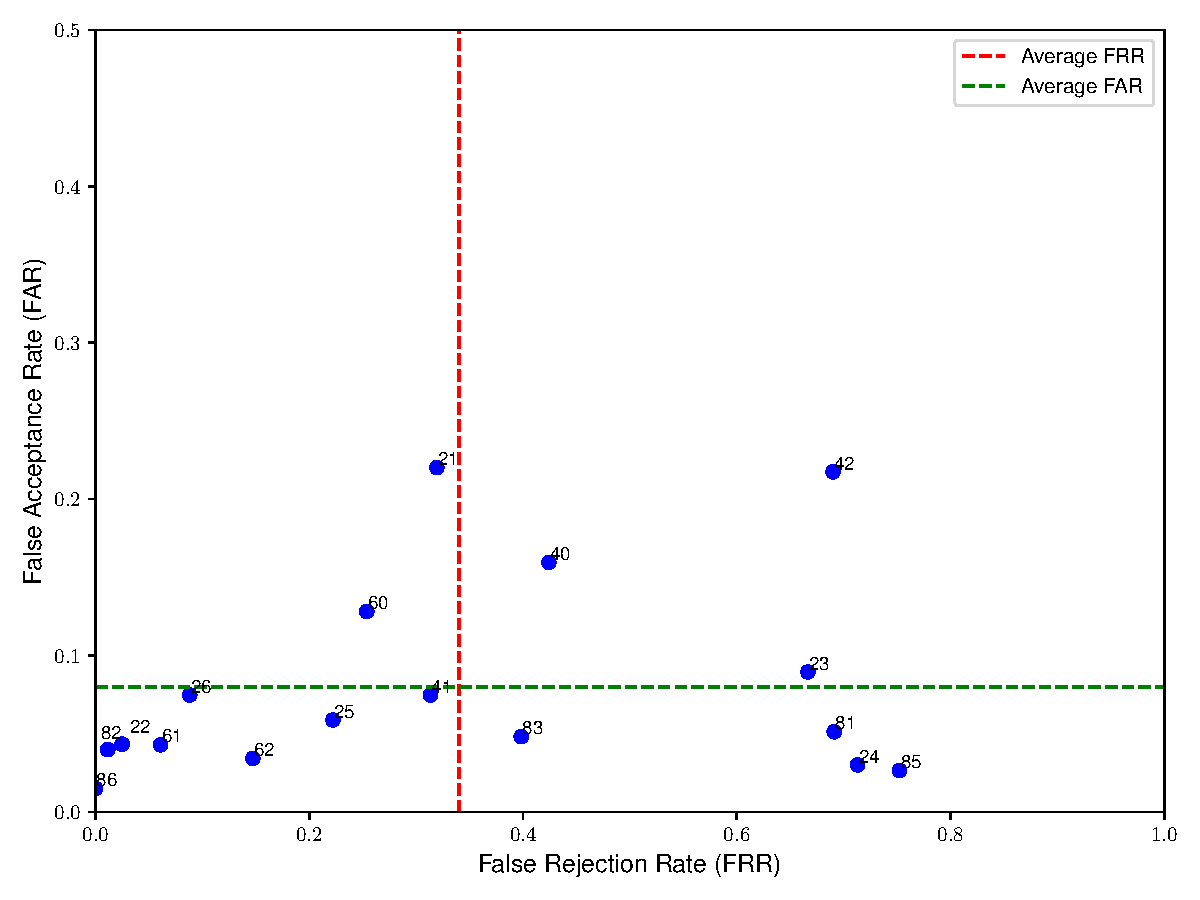
\includegraphics[width=\textwidth]{images/far_vs_frr.pdf} % Replace 'example.pdf' with your PDF file name
	\caption{False acceptance rate vs False rejection rate.}
	\label{fig:frr_vs_far_all_models_base}
\end{figure}

\subsubsection{Confusion matrix for all users}
To evaluate the each model's perofrance, every model was tested on the input of every user. The results of this test are shown in figure \ref{fig:all_models_5_len40}. The values in this matrix represent the procentage of examples classified as positive. It is important to note that the values in this matrix have a diffrent intepretation depending on their position. The values on the diagonal represent the procentage of correctly classified positive example (True Positives) -- the recall of the model. For an ideal classifier these values would equal 100. The values outside the diagonal represent the procentage of incorrectly classied negative examples (False Positves). For an ideal classifier these values would equal 0.

\begin{figure}[H]
	\centering
	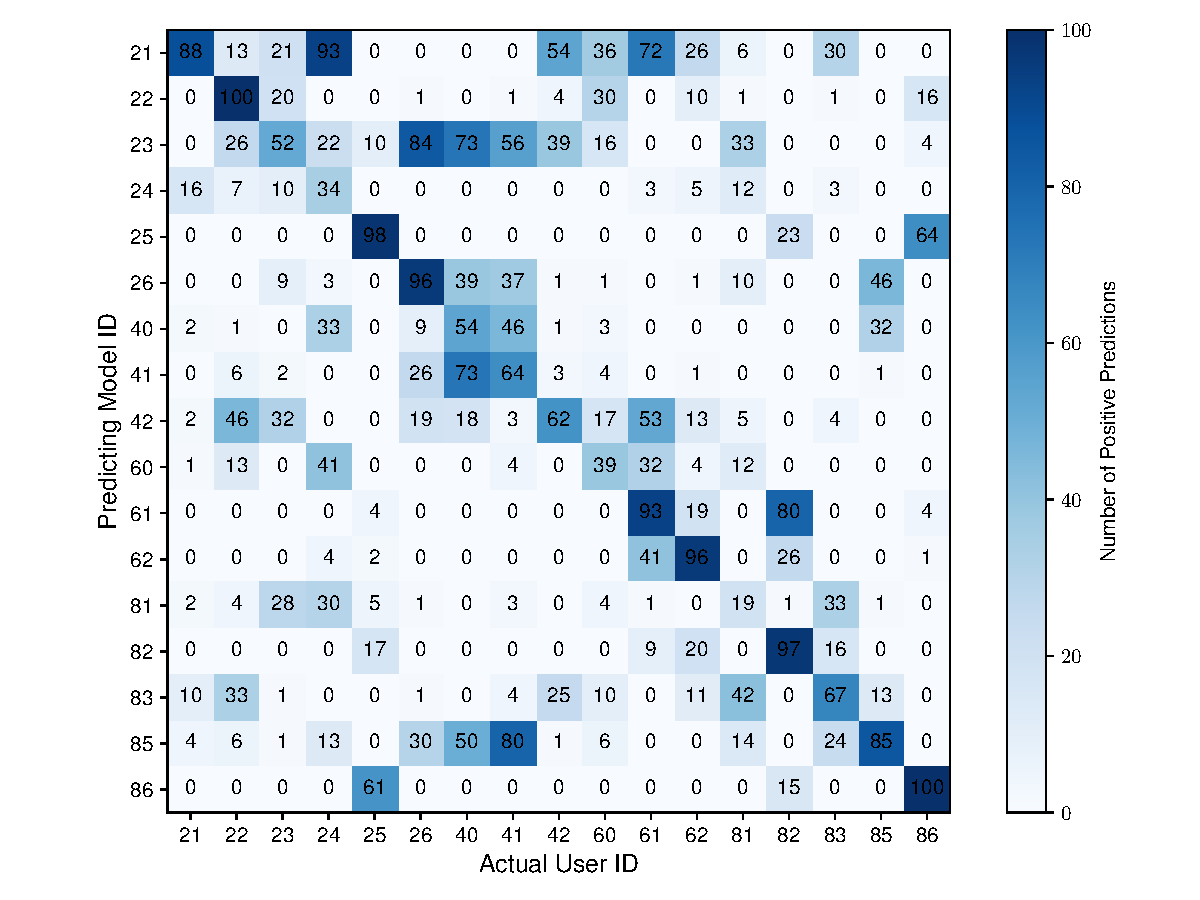
\includegraphics[width=\textwidth]{images/all_models_5_len40.pdf} % Replace 'example.pdf' with your PDF file name
	\caption{Matrix showing the procentage of examples classief as positive for all model--user pairs.}
	\label{fig:all_models_5_len40}
\end{figure}

\myworries{TODO: discuss, possibly with the help of someone else.}

\subsubsection{Equal Error Rate}
We chose to report two diffrent ways to calcualte the equal error rate. To calculate this metric, the decision treshold needs to be adjusted, which can be done globally, for all models or at a per model level. 

The global EER, was calculated to compare the performance of the collection of models to other methods as a whole.
\begin{itemize}
	\item[] Equal Error Rate: 0.157
	\item[] Threshold: 0.20
\end{itemize}
A very low for the decision threshold was neccessary to achive an equal error rate. This suggest that most of the models are rejecting too many positive, and also negative, examples.


The per model EER was calculated by finding equal error rate decision threshold for each model separately. The results are shown in table \ref{table:EER_separate}.

\begin{center}
	\begin{table}[H]
		\begin{center}
			\begin{tabular}{ |c|c|c| } 
				\hline
				User ID & Equal Error Rate & Decision threshold \\
				\hline
				21 & 0.124 & 0.95 \\
				\hline
				22 & 0.026 & 0.95 \\
				\hline
				23 & 0.245 & 0.40 \\
				\hline
				24 & 0.270 & 0.05 \\
				\hline
				25 & 0.037 & 0.85 \\
				\hline
				26 & 0.059 & 0.80 \\
				\hline
				40 & 0.200 & 0.05 \\
				\hline
				41 & 0.081 & 0.35 \\
				\hline
				42 & 0.163 & 0.45 \\
				\hline
				60 & 0.176 & 0.05 \\
				\hline
				61 & 0.066 & 0.80 \\
				\hline
				62 & 0.038 & 0.85 \\
				\hline
				81 & 0.392 & 0.05 \\
				\hline
				82 & 0.026 & 0.95 \\
				\hline
				83 & 0.220 & 0.05 \\
				\hline
				85 & 0.131 & 0.75 \\
				\hline
				86 & 0.028 & 0.90 \\
				\hline
				\hline
				Average & 0.133 & -- \\
				\hline
			\end{tabular}
		\end{center}
		\caption{Per model equal error rate.}
		\label{table:EER_separate}
	\end{table}
\end{center}

\myworries{TODO: the models that do well do VERY well. Some models perform very badly here, well on the FAR vs FRR graph}.


\section{Input features}
This section will compare the impact of input encodings on the final model performance, as measured by the average FAR and FRR, as well as the average per model EER value. The impact of these changes were mesaused by changing only one hyperparameters, while all others remaind the same as shown in table \ref{table:hyperparams}.

\subsection{Input sequance lenght}

\subsection{Character encoding}
\myworries{In tests right now}


\subsection{Egde data encoding}

\begin{center}
	\begin{table}[H]
		\begin{center}
			\begin{tabular}{ |c|c|c|c| } 
				\hline
				Edge encoding method & FAR & FRR & EER \\
				\hline
				\textit{Two dimensional vector of values per node} & 0.069 & 0.666 & 0.395 \\
				\hline
				\textit{Two values per node} & 0.092 & 0.264 & 0.133 \\
				\hline
			\end{tabular}
		\end{center}
		\caption{Comparison of performace with diffrent egde data encoding methods.}
		\label{table:egde_encoding_comp}
	\end{table}
\end{center}

Table \ref{table:egde_encoding_comp} shows the superiority of the \textit{Two values per node} encoding method. While the average far remains comparable, frr, and thus the err, differ by a large amount. This might be cause by the same reasons as the difference between character encoding methods. The method with less aggregation performs worse, as the model might not have seen all possible two letter combinations and failes to generalise.

\subsection{Accelerometer Data}
TLDR doesnt work, comparison for 2 users only - best performing on normal input
Short discussion

\section{Training and model hyperparameters}
\myworries{What goes here ?}

\subsection{Class imbalance}
Another point of experimentation was class balance in the training data. The baseline model was trained on a dataset with two times more positive examples than negative examples. The negative examples were sampled uniformly from all other users, with an offset such that the negative examples for some user were taken from the whole input text. This works for the number of users in the dataset. However, as the number of users grows, and the lenght of input sequence stays fixed, at some point each model needs to be trained only on a subset of the negative class input texts. At that point some models could fail to generalize to unseen negative examples. 
A bigger proportion of possive examples was chosen experimentaly, as it resulted in models that perform better at recognising the positive class.

\begin{center}
	\begin{table}[H]
		\begin{center}
			\begin{tabular}{ |c|c|c|c| } 
				\hline
				Positive to Negative Ratio & FAR & FRR & EER \\
				\hline
				\textit{2:1} & 0.092 & 0.264 & 0.133 \\
				\hline
				\textit{1:1} & 0.080 & 0.340 & 0.177 \\
				\hline
				\textit{1:2} & 0.033 & 0.506 & 0.220 \\
				\hline
			\end{tabular}
		\end{center}
		\caption{Impact of positive to negative ratio on model collection performance.}
		\label{table:egde_encoding_comp}
	\end{table}
\end{center}

While a higher procentage of negative examples were classfied correctly, as indicated by the lower FAR, this comes at the expense of a large drop in the FRR score, to almost half of positive examples being dropped in the case of \textit{1:2} class balance. This means that the collection of models generalised poorly to unseen positive examples, to a degree that would be unacceptable. This can also be seen when comparing the average recall scores across these two collections of models, which droped from \textit{0.7357} to \textit{0.692} and \textit{0.494} when the number of negative examples were doubled. 
\myworries{Cite something, the one i want is paywalled by MIT}
 
However, we also tested training the models with a diffrent positive to negative class ration.
This was motivated by the fact that some models failed to properly recoginise the positive class, 


\myworries{Discuss how positive/negative example ratio had an impact on precission/recall. Maybe note that neg examples were sampled with an offset}

\subsection{Model size}
\myworries{Num of conv layer, layer size etc bigger wasnt better}


\section{Testing model on users}
\myworries{TODO ale chyba nie dla mnie (IW) }

\subsection{TODO title}
\myworries{ TODO: What if we did classify the user on all their input (100 chars). Results would be a n users by n users matrix of 1's and 0's}\\
\myworries{ TOOD: to nie trudne, trzeba wziąc tą nacierz, wybrać treshold, i dać 1 jesli większy 0 jeśli mniejszy}

\subsection{Cross-smartphone user validation}
TODO: what happens if two users train on smartphones that are not their own? What happens, if they cross-use their original model on another phone?
